
\authorsOfDoc{Marcel Rieser}
 
\bigskip

\begin{chapter-intro}
This chapter gives an overview of the major components of MATSim and how they
work together, essentially building the foundation for the MATSim framework.
\end{chapter-intro}

\section{The Major Stages of a MATSim Simulation}

In a typical MATSim simulation, travel demand data is simulated and optimized on
a given transportation network (e.g. a road network, or a multimodal network in
the case when public transport is also considered in the simulation).
The optimization of the demand data is one of the key features of MATSim, making
it suitable to be used for policy studies. In this whole simulation and
optimization process, 5 major stages can be identified:
\begin{itemize}\styleItemize
	\item initial demand
	\item execution
	\item scoring
	\item replanning
	\item analysis
\end{itemize}

These 5 stages are executed in the order shown in
Fig.~\ref{fig:overview:controllerFlow}.
In the following, the responsibilities of each stage is shortly described. The
details for the stages, including what options are available to influence the
stages and how they work, are explained in separate chapters later on.


\begin{figure}[htp]
\begin{center}
  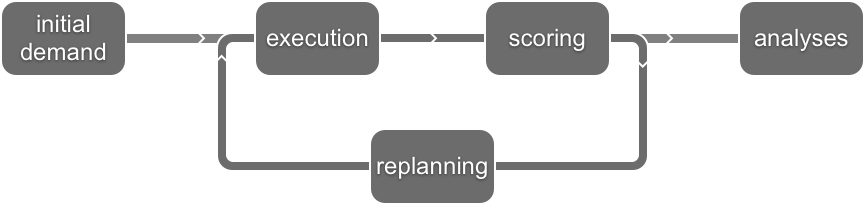
\includegraphics[width=.8\textwidth]{figures/overview/controllerFlow.png}
  \caption{Stages of a MATSim Simulation}
  \label{fig:overview:controllerFlow}
\end{center}
\end{figure}

\paragraph{Initial demand:}
The initial demand describes the mobility behaviour to be simulated. It contains
the full list of agents, and for each agent at least one day plan. A day plan
contains a list of activities (e.g. being \emph{home}, being at \emph{work}) and
trips (e.g. going \emph{by car} to shopping) along with temporal information
(e.g. leaving home \emph{at 7:23 am}, working \emph{until 5:39 pm}) and
additional information (e.g. detailed route going from home to work). Plans
describe the intentions of agents. If agents calculate too optimistically, get
stuck in a traffic jam or miss a bus, it might be that their plan cannot be
realized in the simulation as the agents intended to.

\paragraph{Execution:}
Often also called the \emph{mobility simulation} (or just \emph{mobsim}), the
agents' plans get executed along each other in a representation of the physical
world. This means that the agents and their vehicles are moved around in the
network (the \emph{infrastructure} in the real world). During this execution of
the plans, agents can influence each other by taking up space in the virtual
world. If too many agents want to travel on the same road at a specific time,
they generate a traffic jam in the mobility simulation. This is why the agents'
plans only describe their intentions for a day, but do not actually describe
their day.

\paragraph{Scoring:}
Once the execution of the plans finished, the agents' plans are evaluated based
on their experienced execution. The exact scoring function is customizable, but
generally time spent at activities increases the score, while time spent
travelling decreases it. Agents stuck in a traffic jam thus loose points, while
agents with short and quick trips are able to accumulate more score points by
performing activities for a longer time period.

\paragraph{Replanning:}
As mentioned in the execution stage, agents can be influenced by others and, for
example, get stuck in a traffic jam. During the replanning stage, agents may
modify their plans (actually, they modify copies of the plans, see
Sec.~\ref{sec:Overview:Optimization}) in order to try to avoid situations in the
mobility simulation that lead to bad scores. Typical examples of such
modifications are the modification of activity end times, effectively changing
the start time of the following trip, changing the mode of transport for a trip,
or changing the route for a trip (departure time choice, mode choice, route
choice). In MATSim, these modifications are performed by so-called
\emph{Strategy Modules}.

\paragraph{Analysis:}
At the end of a complete simulation, one is often interested in some key
performance values of the simulation. Examples could be mode shares, miles
travelled in total by all agents, or average trip duration and distance per
mode and hour. Such analyses could either be automatically be performed at then
end, or in a separate post-processing step.

\bigskip

The three stages Execution, Scoring and Replanning are performed iteratively in
order to give the agents multiple opportunities to adapt their plans to the
plans and behaviour of the other agents. This is why MATSim typically performs
multiple \emph{iterations} within one simulation run, consisting of multiple
mobility simulation, scoring and replanning executions, until the end result is
available.

MATSim provides a \emph{Controller} (sadly misspelled as \emph{Controler} in
some places) which implements the iteration loop as shown in
Fig.~\ref{fig:overview:controllerFlow}. This Controller is typically the entry
point for running MATSim simulations, as it handles all aspects from loading all
the required data, configuring the whole setup according to the user's settings,
and iteratively calling the execution, scoring and re-planning stages.
Chpt.~\ref{sec:Running} shows the usage of the Controller in more
detail.


\section{The Optimization Process}
\label{sec:Overview:Optimization}

As outlined above, agents can modify the plans from the initial demand to try to
come up with new variants of the plan that lead to higher scores. The main
concept of the optimization process follows the principles of so-called
\emph{(co-)evolutionary algorithms}. Evolutionary algorithms typically maintain
a set of candidates which are evaluated using a fitness function. New candidates are
generated and evaluated. If they have a bad fitness, they are discarded. If they
have a good fitness, another candidate with a worse fitness is removed from the
set of candidates and the new candidate is added to the set. This is repeated
until no new good candidates are found after some tries.

MATSim implements an evolutionary algorithm for each agent. As all agents are
optimized using their own evolutionary algorithm, the whole system is called a
co-evolutionary algorithm. The set of candidates corresponds to the set of plans
each agent has. New candidates are generated in the replanning stage by making a
copy of an existing plan and modifying the copy. The fitness evaluation is done
by scoring the execution of the plan.
Thus, the replanning stage in MATSim corresponds to the generation of new
candidates of evolutionary algorithms, while the execution and scoring of plans
corresponds to the evaluation of the fitness of the candidates. The repetition 

With each iteration, the goal is that the average score of the executed plans
increase, corresponding to the agents improving their plans such that they can
perform their daily activities as good as possible.
Fig.~\ref{fig:overview:scores} shows how the average score develops in a typical
MATSim simulation over the course of the iterations. Note that the absolute
value of the scores may depend upon the scenario. As can be nicely seen in the
figure, the average executed score typically improves very rapidly in the first
few iterations, but will only improve very slightly in later iterations or even
degrade a few times.


\begin{figure}[htp]
\begin{center}
  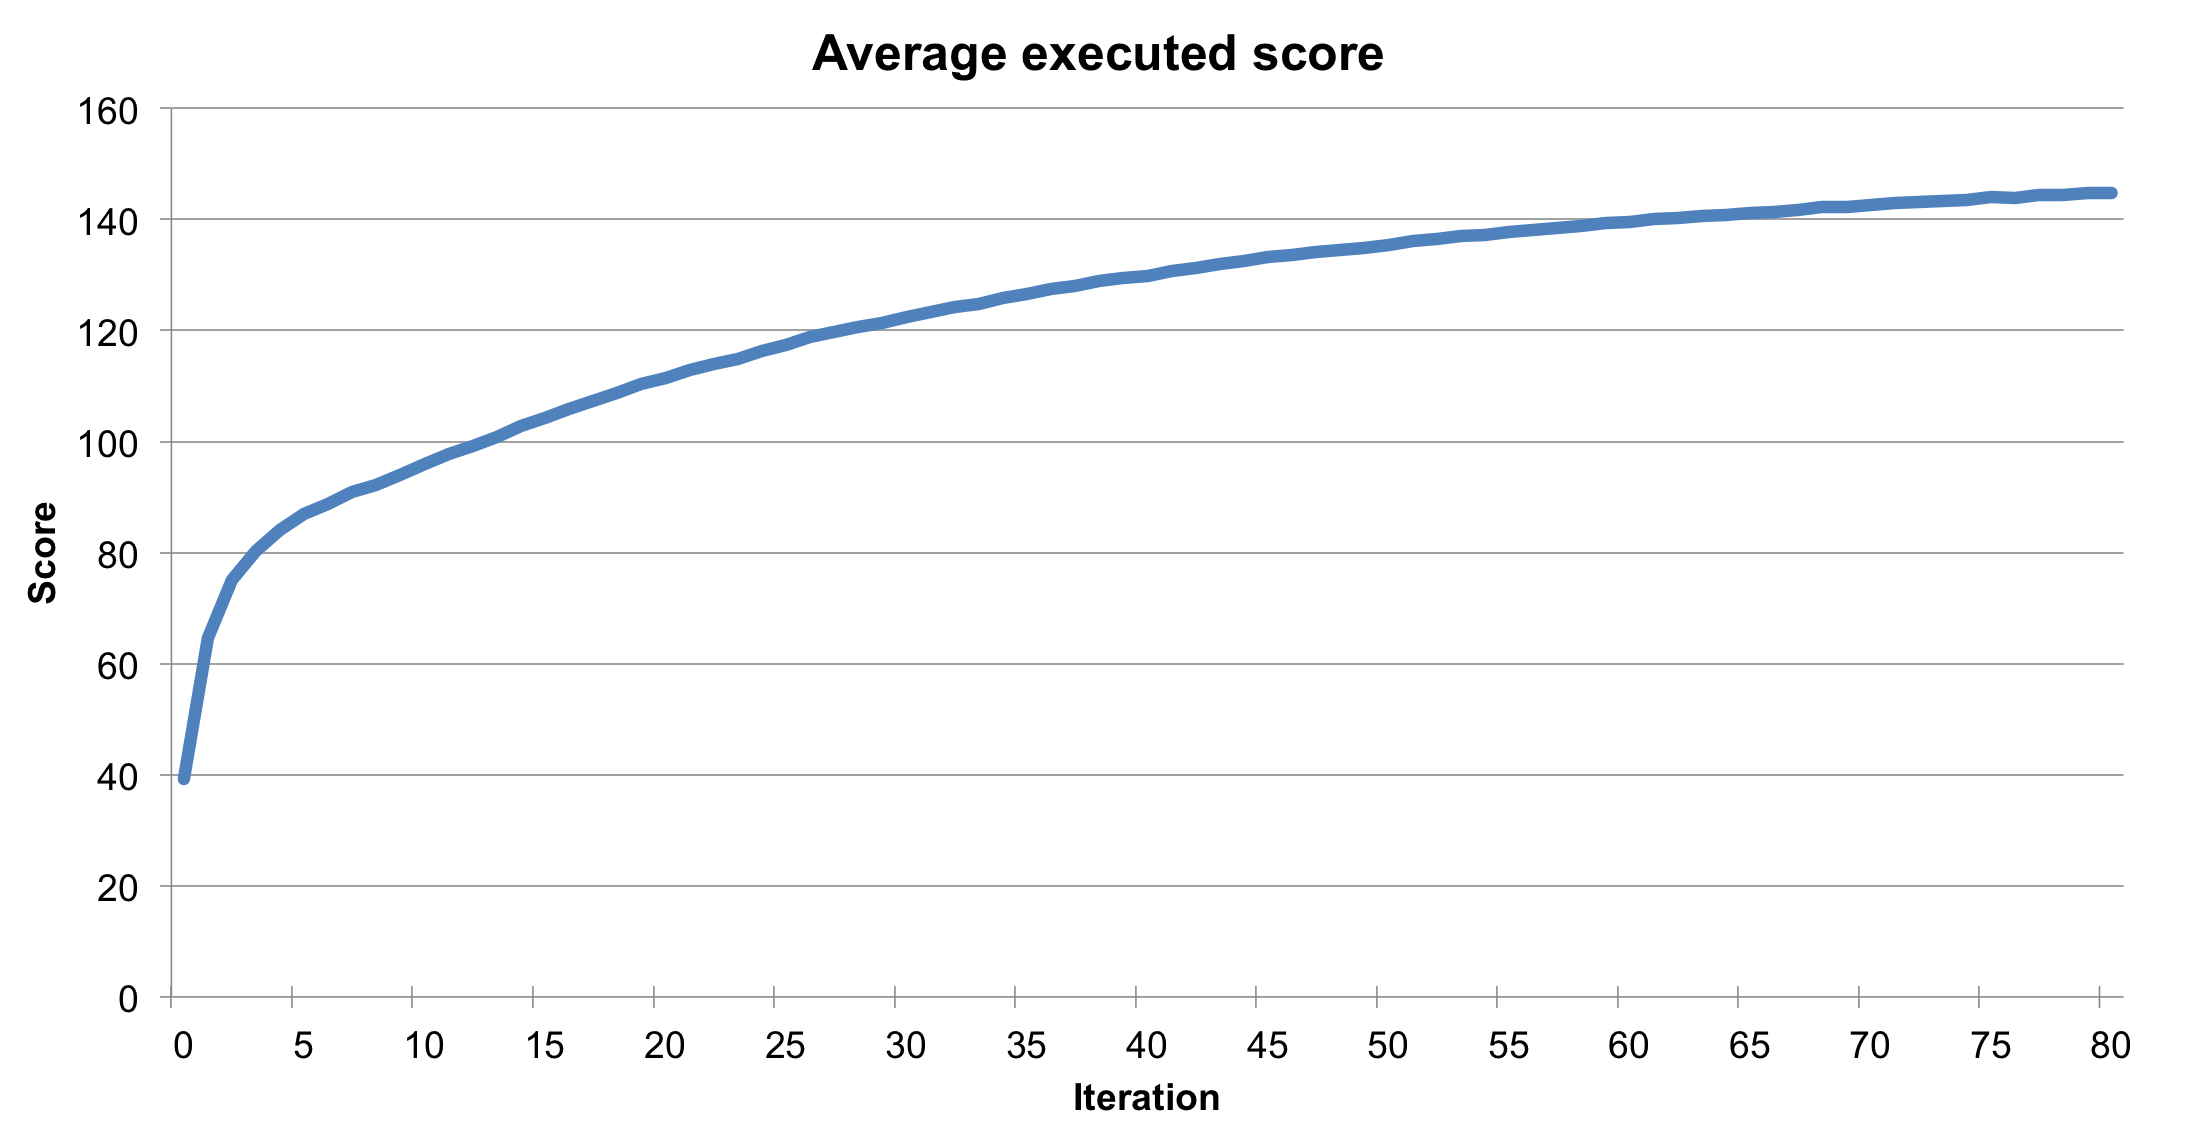
\includegraphics[width=.9\textwidth]{figures/overview/scorestats.png}
  \caption{Tpyical development of the average score of the executed plans over
  the iterations}
  \label{fig:overview:scores}
\end{center}
\end{figure}


\section{Mobility Simulation Events}
The mobility simulation moves the agents around in the virtual world according
to their plans and within the bounds of the ``simulated reality''. The
mobility simulation documents its moves with so-called ``Events''. These events
are small pieces of information describing the action of an object at a
specific time. Examples of such events can be:
\begin{itemize}\styleItemize
  \item An agent finishes an activity
  \item An agent starts a trip
  \item A vehicle enters a road segment
  \item A vehicle leaves a road segment
  \item An agent bordes a public transport vehicle
  \item An agent arrives at a location
  \item An agent starts an activity
\end{itemize}
Each event has a timestamp, a type, and additional attributes required to
describe the action like the agent's id, a link id, an activity type or other
data. In theory, it should be possible to replay the mobility simulation just by
the information stored in the events. While plans describe the agents' plan for
a day, the events describe how the agents' day actually was (according to the
simulation).

As the events are so basic, each agent typically generates hundreds of events
during one execution of a mobility simulation. In total, the number of events
generated by a mobility simulation can easily reach a million or more, with
large simulations even generating more than a billion events. But as the events
really describe all the details from the execution of the plans, it is possible
to extract mostly any kind of aggregated data one is interested in. Practically
all analyses of MATSim simulations make use of events to calculate some data.
Examples of such analyses are the average duration of an activity, average trip
duration or distance, mode shares per time window, number of passengers in
specific transit lines and many more.

The scoring of the executed plans makes use of events to find out how much time
agents spent at activities or for travelling. Some replanning modules might
make use of events as well: The router for example can use the information
contained in events to figure out what links are jammed at certain times and
route agents around that jam when creating new plans.


\section{Customizability}
MATSim is designed to be modular. Nearly all parts can be customized, replaced
or enhanced with custom functionality. Some customizations are easier than
others. Replacing the mobility simulation for additional behaviour might be one
of the hardest things to achieve, because a lot of functionality would have to be re-implemented. Changing the replanning on the other hand is
quite easy, especially as there is already a number of modules available for
different replanning needs which can be activiated and used without programming
and only by modifying the configuration file. This guide will mostly focus on
functionality available in a standard release of MATSim that can be used just by
making changes to the configuration file, and not on enhancing MATSim by
programming custom functionality.


\begin{note}
In order to work with MATSim, you should know the \emph{5 major stages} of a
MATSim simulation, why MATSim uses \emph{iterations} and understand conceptually what
data is contained in \emph{plans} and what data is contained in \emph{events}.
\end{note}
